\chapter{Simulation Setup and Configuration}
\label{ch:SimulationSetupConfiguration}

For testing \ac{glosa} schemes at the signalized \emph{Neckartor} junction, this chapter sets up a standard way to do experiments. The investigation employs a microscopic network developed in \ac{sumo} and controlled via the \ac{traci} interface. This digital twin accurately replicates the junction's lane geometry, \ac{spat} phasing, and local diesel-ban regulations. Synthetically generated traffic demand, anchored to measured flow data, spans a wide range of conditions from free-flow to oversaturation.
\mynewline
The chapter is organized into three main sections. Section~\ref{sec:SimEnvironment} outlines the simulation environment, including the network configuration, vehicle fleet composition, \ac{eidm} parameters, and the emission logging setup. Section~\ref{sec:exec_protocol} specifies the execution protocol, which systematically varies traffic flow, \ac{glosa} market penetration, communication range, and other key parameters such as the slack time, \gls{tslack}. Finally, Section~\ref{sec:performance_evaluation} defines the performance metrics used for evaluation, including vehicle stop counts, mean speed, fuel consumption, pollutant emissions, and break-even penetration rates.

\section{Simulation Environment}
\label{sec:SimEnvironment}

The experimental investigation is conducted using the open-source \ac{sumo} framework, selected for its high-fidelity microscopic vehicle dynamics and its capacity for deterministic reproducibility. All simulation inputs are provided via static configuration files to ensure consistency, with no on-line calibration performed during the runs. The platform's default numerical integration solver is used for all calculations.
\mynewline
The simulation network is a high-fidelity digital twin of the signalised \emph{Neckartor} junction in Stuttgart, a location known for heavy traffic and previous environmental studies. Figure~\vref{fig:NeckartorMapComparison} provides a direct visual comparison of the junction. The satellite imagery in Figure~\vref{fig:NeckartorMapReal} shows the complex real-world geometry, which is precisely replicated in the \ac{sumo} environment, as depicted in Figure~\vref{fig:NeckartorMapSUMO}. This includes all lane layouts and dedicated turn pockets. Signal control is governed by fixed \ac{spat} and \ac{map} plans extracted from the actual roadside controller, which are assumed to be invariant throughout each simulation run. In accordance with local traffic regulations, the vehicle fleet excludes diesel vehicles that do not meet the Euro 6 standard, mirroring the driving ban on older, more polluting models. The simulation's traffic demand is anchored to empirical data, with measured vehicle counts from 2023 indicating a peak flow of $2800\unit{\veh\per\hour}$.
\mynewline

\begin{figure}[htb]
  \centering
  \begin{subfigure}[b]{0.49\textwidth}
    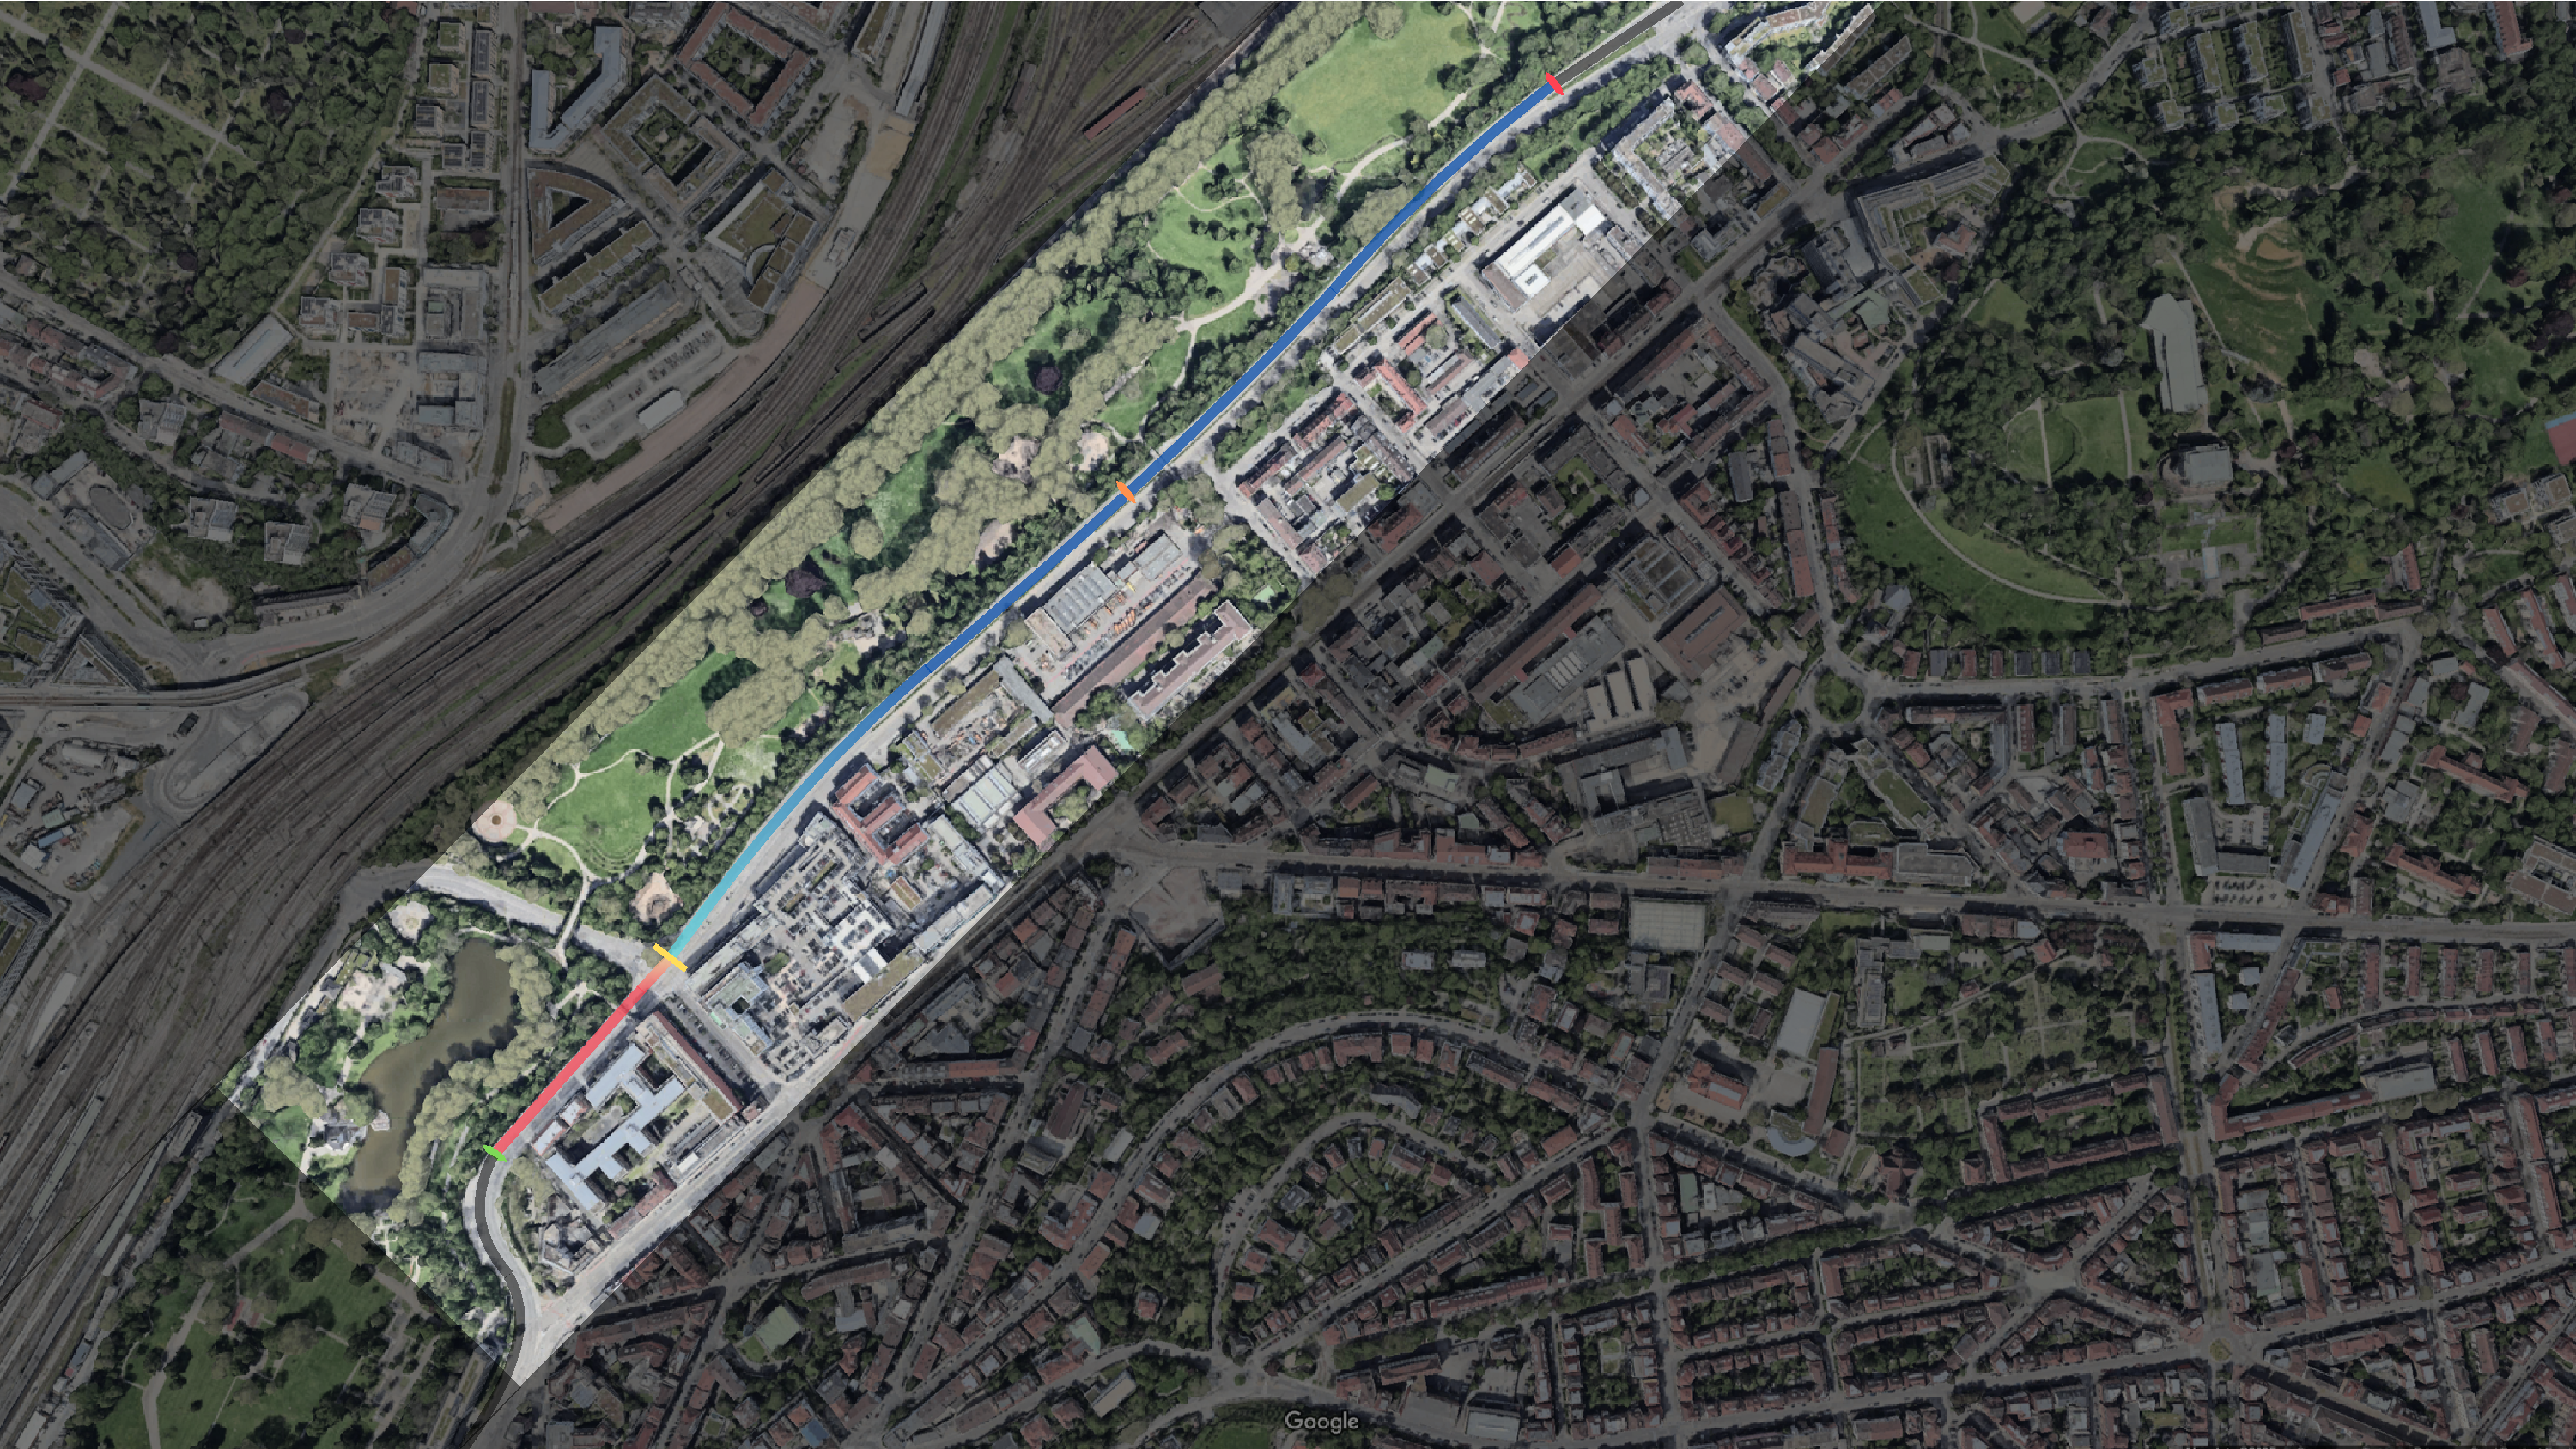
\includegraphics[width=\linewidth, page=1]{data/img/Neckartor/StuttgartNeckartorReal.pdf}
    \caption[Neckartor junction satellite image]{Satellite imagery of the real-world Neckartor junction in Stuttgart, highlighting the complex geometry and surrounding urban environment.}
    \label{fig:NeckartorMapReal}
  \end{subfigure}
  \hfill
  \begin{subfigure}[b]{0.49\textwidth}
    \includegraphics[width=\linewidth, page=1]{data/img/Neckartor/StuttgartNeckartorSumo.pdf}
    \caption[Digital twin of Neckartor in \ac{sumo}]{The digital twin of the Neckartor junction as implemented in the \ac{sumo} environment, showing the modelled lanes and connections.}
    \label{fig:NeckartorMapSUMO}
  \end{subfigure}
  \caption[Real-World vs. Simulated Neckartor Junction]{%
  Comparison of the real-world Neckartor junction (left) with its high-fidelity digital twin in the \ac{sumo} simulation (right). 
  The red segment marks the downstream cordon, while the blue segment indicates the upstream cordon. 
  The yellow line represents the signalized intersection. 
  Red square dots denote the start points for the $1000\unit{\metre}$ downstream advisory range, while orange square dots denote the start points for the $500\unit{\metre}$ range. 
  The green square marks the corresponding upstream end point of each advisory range. 
  Yellow arrows indicate the driving direction in each lane.}
  \label{fig:NeckartorMapComparison}
\end{figure}

Traffic demand is generated synthetically but is anchored to real-world loop detector data from the B14 corridor. The generated flow levels span the full spectrum of traffic states, from light, uncongested conditions to heavy, oversaturated congestion. Within each scenario, vehicles are introduced into the network with uniform inter-arrival times. Route assignment follows an equal probability distribution across all legitimate movements to ensure a balanced saturation of all lane groups. The \ac{glosa} \ac{mpr} is treated as a primary experimental variable, systematically tested in $10\%$ increments from $0\%$ (no equipped vehicles) to $100\%$ (fully equipped fleet). To manage this, two statistically independent insertion streams are used, allowing \ac{glosa}-equipped and non-equipped vehicles to coexist and interact within the same network environment.
\mynewline
The longitudinal driving behaviour for all vehicles is governed by the \ac{eidm}, a model chosen for its demonstrated ability to realistically capture stop-and-go waves and queue discharge dynamics. To ensure the simulation reflects real-world driver diversity, a heterogeneous fleet is synthesized by defining a combination of eleven fixed and eleven variable vehicle parameters. The fixed parameters, which establish baseline physical and behavioural constraints for all vehicles, are detailed in Table~\vref{tab:FixedFleetParams}. The variable parameters, listed in Table~\vref{tab:VariableFleetParams}, are sampled independently of uniform distributions over their specified ranges for each vehicle at spawn time. This methodology produces a rich vehicle population with a plausible span of physical dimensions (e.g., length and width) and driver characteristics (e.g., aggressiveness, reaction time), preventing a bias towards any single calibration point.
\mynewline

\begin{table}[htb]
  \centering
  \caption[Variable Vehicle Fleet Parameters]{Variable vehicle parameters used to synthesize the heterogeneous fleet in \ac{sumo}. Each parameter is drawn independently of a uniform distribution over the specified range at vehicle spawn time to ensure a realistic mix of driver behaviours and vehicle types. Derived from Lenz \cite{Lenz2024}.}
  \label{tab:VariableFleetParams}
  \resizebox{\textwidth}{!}{%
    \begin{tabular}{l l c c}
      \toprule
      \textbf{Parameter} & \textbf{Explanation} & \textbf{Min Value} & \textbf{Max Value} \\
      \midrule
      minGap & Minimum vehicle gap at standstill & $0.5\unit{m}$ & $4\unit{m}$ \\
      accel & Maximum acceleration & $0.97\unit{m\,s^{-2}}$ & $4\unit{m\,s^{-2}}$ \\
      startupDelay & Time delay until vehicle starts moving & $0.0\unit{s}$ & $2.0\unit{s}$ \\
      tau & Time headway maintained to the preceding vehicle & $0.5\unit{s}$ & $1.5\unit{s}$ \\
      delta & Influences how the vehicle reacts to speed differences & $1.0$ & $4.97$ \\
      treaction & Driver's reaction time & $0.2\unit{s}$ & $0.9\unit{s}$ \\
      tacmax & Time the vehicle needs to reach maximum acceleration & $0.5\unit{s}$ & $3.0\unit{s}$ \\
      Mflatness & \enquote{Flatness} of the acceleration and deceleration behavior & $1.0$ & $5.0$ \\
      Mbegin & Parameter for starting behavior & $0.1$ & $1.49$ \\
      length & Length of the vehicle & $2.2\unit{m}$ & $9.3\unit{m}$ \\
      width & Width of the vehicle & $1.5\unit{m}$ & $2.5\unit{m}$ \\
      \bottomrule
    \end{tabular}%
  }
\end{table}

\begin{table}[htb]
  \centering
  \caption[Fixed Vehicle Fleet Parameters]{Fixed vehicle parameters shared by all vehicles in the simulation fleet. These values define baseline behaviours and physical constraints, ensuring consistent dynamics across the entire population. Derived from Lenz \cite{Lenz2024}.}
  \label{tab:FixedFleetParams}
  \resizebox{\textwidth}{!}{%
    \begin{tabular}{l l c}
      \toprule
      \textbf{Parameter} & \textbf{Explanation} & \textbf{Value} \\
      \midrule
      decel & Maximum deceleration & $2.5\unit{m\,s^{-2}}$ \\
      emergencyDecel & Maximum emergency braking deceleration & $15\unit{m\,s^{-2}}$ \\
      tpreview & Time horizon a vehicle "looks" into the future to plan speed & $4\unit{s}$ \\
      tPersDrive & Duration the vehicle remains in continuous driving mode & $3\unit{s}$ \\
      tPersEstimate & Duration the vehicle remains in estimation mode & $10\unit{s}$ \\
      coolness & Influences how calmly or aggressively a vehicle reacts to disturbances & $0.99$ \\
      signaleader & Inaccuracy of speed adaptation to the preceding vehicle & $0.02$ \\
      sigmaerror & Inaccuracy regarding errors in driving style (speed, distance) & $0.1$ \\
      sigmagap & Inaccuracy of the gap to the preceding vehicle & $0.1$ \\
      jerkmax & Maximum rate of change of acceleration & $3\unit{m\,s^{-3}}$ \\
      epsilonacc & Inaccuracy of acceleration estimation & $1.0$ \\
      \bottomrule
    \end{tabular}%
  }
\end{table}

Each simulation is run for a total temporal horizon of $43.33\unit{min}$. The initial $10\unit{min}$ of this period serves as a warm-up phase, which allows traffic flows to stabilize and ensures that initial transient effects do not influence the results. Consequently, only data from the final $33.33\,\unit{min}$ are used for statistical analysis. A simulation time step of $0.1\unit{s}$ is maintained to provide sufficient resolution for both the \ac{eidm}'s dynamic equations and for the accurate integration of instantaneous emissions. For data collection, the analysis is spatially constrained to a corridor extending $1\unit{km}$ upstream and $200\,\unit{m}$ downstream from the intersection's primary stop line. This spatial clipping focuses the evaluation on the region most directly influenced by the \ac{glosa} advisories.
\mynewline
For each simulated vehicle, a dedicated log file is generated that records a high-resolution time series of its state, including timestamp, position, speed, and acceleration. Instantaneous emission rates for all relevant pollutants are concurrently calculated using \ac{sumo}’s internal emission model back-ends. To facilitate post-processing with external analysis scripts, these logs are flushed at every simulation step. A consistent configuration is applied across all scenarios to ensure the comparability of results throughout the comprehensive sweeps of traffic flow, market penetration, and other experimental parameters.



\section{Execution Protocol and Parameterization}
\label{sec:exec_protocol}

The execution protocol translates the conceptual design into a reproducible set of simulation runs that sample all relevant boundary conditions while keeping computational cost within practical limits. Reproducibility is guaranteed by fixing the random seed to \texttt{12345}; thus every pseudo-random operation like route choice, lane assignment, and vehicle parameter draw, yields identical sequences across repeated executions. Each run evaluates one of two \ac{glosa} algorithm variants: (i) the \emph{baseline} or \emph{flow-optimised} controller, which targets minimum delay, and (ii) the \emph{eco-driving} controller, which minimises fuel use but ignores explicit queue effects. For every algorithm, the parameter sweep enumerates all combinations of traffic flow, market penetration, and communication range, leading to $176$ distinct scenarios per controller and hence $352$ in total. An overview of all the parameters is given in Table \ref{tab:ScenarioMatrix}. The three independent factors are detailed below.  

\begin{enumerate}
\item \textbf{Traffic flow.} Eight demand levels are enforced by limiting the number of inserted vehicles to 50, 100, 250, 500, 1000, 1500, 2000, and 2500, corresponding to 69, 138, 346, 692, 1385, 2077, 2769, and 3462\,veh\,h\(^{-1}\), respectively.  
\item \textbf{Market penetration.} The \ac{glosa} \ac{mpr} varies from 0\,\% to 100\,\% in 10-percentage-point increments. A Bernoulli draw at spawn time classifies each vehicle as equipped or non-equipped, producing two statistically independent traffic streams within the same macroscopic flow.
\item \textbf{Communication range.} Prior work by Lenz \cite{Lenz2024} found no statistically significant difference between 500\,m and 1000\,m communication horizons; therefore only the 500\,m radius is tested here but retained as a formal factor to keep the full Cartesian design consistent with earlier literature. The advisory is sent whenever an equipped vehicle’s distance to the stop line is $\gls{dup}\leq500\,\mathrm{m}$ and $\gls{ddown}\leq200\,\mathrm{m}$.
\end{enumerate}

All other settings are held constant across the sweep. The optimiser assumes an additional fixed switch time of 2.1\,s to capture actuation delays between the traffic controller and the actual signal head. Slack time \(\gls{tslack}\) is sampled uniformly in the closed interval \([0.1,5]\,\mathrm{s}\) at run time, reflecting uncertainty in residual phase duration. Downstream distance is clipped to 200\,m, matching the evaluation window specified in Section~\ref{sec:SimEnvironment}. A yellow-phase buffer of \(0.5\,\mathrm{s}\) prevents infeasible trajectories that might straddle the amber interval. The numerical search increment for the longitudinal optimiser, \(\Delta a\), is fixed to \(0.01\,\mathrm{m\,s^{-2}}\); preliminary tests confirmed that smaller steps add negligible accuracy but inflate computation time. Objective-function weights follow \(\alpha_{\text{speed}}=1.0\) and \(\alpha_{\text{reach}}=0.5\). Speed estimation downstream uses one-second velocity samples, which balances responsiveness with noise suppression.
\mynewline
Emissions and energy demand are assessed with two fuel models, \ac{hbefa} 4 and \textsc{PHEMlight} 5, specified in section \ref{subsubsec:detailed_emission_models}. Queue length is forcibly set to zero in all optimiser calls, thereby isolating pure speed-advice effects from more complex queue-estimation feedback loops.

\begin{table}[tbp]
  \centering
  \caption{Scenario design matrix per algorithm.  Each cell is executed once with seed~\texttt{12345}.}
  \label{tab:ScenarioMatrix}
  \begin{tabular}{ccccc}
    \toprule
    Factor & Symbol & Levels & Values & Unit \\
    \midrule
    Traffic flow & \(Q\) & 8 & 69–3462 & veh\,h\(^{-1}\) \\
    Market penetration & MPR & 11 & 0–100 (step 10) & \% \\
    Comm.\ range & \(r_{\text{com}}\) & 2 & 500, 1000 & m \\
    \midrule
    \multicolumn{2}{c}{Total scenarios} & \multicolumn{3}{c}{\(8\times11\times2=176\)}\\
    \bottomrule
  \end{tabular}
\end{table}

The optimizer assesses potential speed profiles within the specified communication range of 500 meters prior to and 200 meters following the intersection during runtime. Upstream motion is constrained by the extended \ac{eidm} envelope described in Section~\ref{sec:SimEnvironment}. The controller solves a univariate line search over acceleration \(a_{\text{up}}\) with step \(\Delta a\). Terminal conditions are checked at the downstream horizon \(l=200\,\mathrm{m}\); trajectories violating \(\gls{vmin}\) or \(\gls{bmax}\) are discarded. 
\mynewline
The resulting dataset underpins all metrics specified in Section~\ref{sec:performance_evaluation}. Because the protocol controls every stochastic degree of freedom and stores exhaustive logs, future researchers can reproduce the study by re-running the same configuration files and seed. Any deviation, such as a different communication horizon or an additional queue-aware variant, would simply append new factors to the Cartesian design while preserving the core template documented here.


\section{Performance Metrics and Evaluation Methodology}
\label{sec:performance_evaluation}

The assessment framework is designed to expose the trade-off between smoother traffic flow and ecological benefit introduced by the two \ac{glosa} variants. All quantities are derived from the trajectory and emission logs produced by \ac{sumo}. Each scenario is executed exactly once with a fixed random seed, yielding a single deterministic outcome; therefore, statistical confidence intervals are not applicable.

\paragraph{Microscopic Traffic Efficiency.}
The quality of longitudinal driving behaviour is quantified using four primary indicators:

\begin{enumerate}[label=\textbf{(\roman*)}]
    \item \textbf{Stops per Vehicle:} The stop frequency, \gls{nstop}, is a key metric for traffic disruption. A stop is defined as an event where a vehicle's speed drops below a threshold of $2\unit{\metre\per\second}$ after having been above it. For a single vehicle $i$, the total number of stops is calculated as:
    \begin{equation}
        N_{\mathrm{stop},i} = \sum_{k=2}^{K}{\mathbbm{1}}(v_{i,k} < 2 \land v_{i,k-1} \ge 2)
    \end{equation}
    The scenario average, $\bar{N}_{\mathrm{stop}}$, is the mean of this value over all $N$ vehicles.

    \item \textbf{Mean Vehicle Speed:} The average speed, $\bar{v}$, serves as a measure of overall network mobility and is computed over all vehicles and all recorded time steps:
    \begin{equation}
        \bar{v} = \frac{1}{NK}\sum_{i=1}^{N}\sum_{k=1}^{K} v_{i,k}
    \end{equation}

    \item \textbf{Mean Absolute Acceleration:} As a surrogate for passenger comfort and powertrain strain, the mean absolute acceleration is calculated as:
    \begin{equation}
        \overline{|a|} = \frac{1}{NK}\sum_{i=1}^{N}\sum_{k=1}^{K} |a_{i,k}|
    \end{equation}

    \item \textbf{Mean Absolute Jerk:} To quantify the smoothness of acceleration changes, the mean absolute jerk, \gls{j}, is computed. Lower values indicate smoother, more comfortable driving profiles.
    \begin{equation}
        \overline{|j|} = \frac{1}{NK}\sum_{i=1}^{N}\sum_{k=1}^{K} |j_{i,k}|
    \end{equation}
\end{enumerate}

\paragraph{Macroscopic Throughput.}
Throughput is quantified by the mean number of vehicles crossing the intersection's stop-line detector per signal cycle. For a cycle length of $T_{\mathrm{cycle}}=120\unit{\second}$ with two green intervals, $I_{1}=[2,35]\unit{\second}$ and $I_{2}=[62,96]\unit{\second}$, the number of vehicles $N_{c}$ detected during cycle $c$ is:
\begin{equation}
    N_{c} = \#\lbrace i : t_{i,\mathrm{detection}} \in I_{1} \cup I_{2} \rbrace
\end{equation}
where $t_{i,\mathrm{detection}}$ is the time vehicle $i$ is detected at the stop line. The average per-cycle throughput is then $\overline{N}_{\mathrm{cycle}} = \frac{1}{C}\sum_{c=1}^{C} N_{c}$.

\paragraph{Energy Demand and Pollutant Emissions.}
The environmental impact is characterised by per-vehicle pollutant rates, with \ac{co2} as the primary metric for fuel consumption. Emissions are computed over the $1.2\unit{\kilo\metre}$ evaluation corridor by summing the instantaneous rates in the log, multiplying by the time step $\Delta t = 0.1\unit{\second}$, and normalising by distance:
\begin{equation}
    e_{i} = \frac{1}{1000 \cdot L} \sum_{k=s_i}^{e_i} \dot{m}^{\mathrm{CO_2}}_{k} \cdot \Delta t, \quad \text{where } L = 1.2\,\mathrm{km}
\end{equation}
The same form applies to \ac{nox} emissions. The analysis is performed in parallel for both the HBEFA4 and PHEMlight5 emission models.

\paragraph{Relative Performance and Break-Even Analysis.}
To facilitate comparisons, each metric $y$ is expressed as a percentage deviation from the uncontrolled baseline (0\% \ac{mpr}). A break-even analysis is conducted by directly comparing the performance of the \ac{eco-glosa} and \ac{flow-glosa} controllers at each discrete combination of traffic flow and \ac{mpr}. This identifies which controller provides a superior outcome under specific conditions.

\paragraph{Computational Viability.}
The practical feasibility of each algorithm is assessed by recording and comparing the absolute wall-clock time required to complete each simulation scenario. The incremental cost of the eco-driving algorithm is evaluated by comparing its runtime, $T_{\mathrm{traci,eco}}$, against that of the less complex flow-optimised baseline, $T_{\mathrm{traci,flow}}$.

\paragraph{Visualisation Strategy.}
The results are conveyed using a harmonised set of graphical summaries:
\begin{enumerate}[label=\textbf{(\alph*)},leftmargin=*]
    \item \textbf{Line Charts:} Key metrics such as mean speed, stop frequency, and \ac{co2} emissions are plotted as functions of \ac{mpr}. Each traffic demand level is shown in a separate panel to facilitate direct comparison across different levels of congestion.
    \item \textbf{Heat Maps:} The relative performance difference in \ac{co2} emissions between the two controllers is displayed on a two-dimensional grid of traffic flow versus penetration rate. This provides a clear overview of the operating regimes where each strategy delivers a net environmental benefit.
    \item \textbf{Break-Even Boundary:} On the 2D heat maps, the break-even penetration rate, $p^{\star}$, is traced as a boundary line. The line is solid black where the performance crossover is clear and decisive, and a dashed gray line where the transition is ambiguous or the performance difference is negligible.
\end{enumerate}
As each data point is derived from a single deterministic simulation run, no statistical error bars are presented.

\paragraph{Interpretation Focus.}
The subsequent analysis of results concentrates on two primary objectives: (i) to quantify the absolute and relative reductions in \ac{co2} emissions achieved by the eco-driving algorithm, and (ii) to identify the specific penetration-demand corridors where these ecological benefits can be achieved without significantly degrading traffic throughput. By normalizing all performance metrics against a baseline and indexing them by market penetration, this evaluation methodology yields transparent and scalable insights, ensuring the findings provide a robust foundation for future work involving new algorithms or network geometries.
\mynewline
The remainder of this chapter is dedicated to a detailed discussion of these results, structured by the key performance indicators. Section~\vref{sec:Results_GreenPhaseFlow} begins by evaluating the intersection's macroscopic throughput. The analysis then moves to microscopic traffic efficiency, examining the average vehicle speed in Section~\vref{sec:Results_MeanSpeed} and the vehicle stop frequency in Section~\vref{sec:Results_Stops}. Driving smoothness is assessed in Section~\vref{sec:Results_Smoothness} by analysing both the mean absolute acceleration and mean absolute jerk. Subsequently, Section~\vref{sec:Results_Emissions} details the environmental impact, focusing on \ac{co2} and \ac{nox} emissions. The core trade-offs are synthesised in Section~\vref{sec:Results_BreakEven}, which presents the break-even analysis. Finally, the practical feasibility is evaluated in Section~\vref{sec:Results_Computational} by comparing the computational runtimes of the two algorithms.
